\chapter{Codifica}
\label{cap:codifica}

\intro{Il presente capitolo illustra l'organizzazione del codice prodotto e i dettagli implementativi della soluzione di telemetria, riprendendo le scelte progettuali descritte nel capitolo~\ref{cap:progettazione} e mostrando come si traducono nella struttura effettiva del framework \emph{Sia.Server.Framework}.}\\

\section{Organizzazione del codice}

Il codice di telemetria è distribuito su due livelli del framework:

\begin{itemize}
    \item un livello \textbf{condiviso} (\texttt{Application.Shared.Telemetry} e
        \texttt{BaseApplicationBuilder}), che configura il pipeline \gls{otel},
        registra \emph{sampler}, \emph{processor} e \emph{exporter}, e definisce le
        convenzioni comuni (attributi di \emph{resource}, \emph{middleware}
        di arricchimento utente);
    \item un livello \textbf{per-modulo} (\texttt{Sia.\{Modulo\}/Diagnostics/}), che contiene
        la classe statica \texttt{Sia\{Modulo\}Diagnostics} con \texttt{ActivitySource},
        \texttt{Meter}, \texttt{Counter}, \texttt{Histogram}, e la dashboard Grafana
        \texttt{\{nome\}.dashboard.json} versionata insieme al codice.
\end{itemize}

Questa suddivisione garantisce che un nuovo modulo, per integrare la telemetria, debba solo
creare la propria classe \texttt{Diagnostics} e registrare il proprio \texttt{Meter} e
\texttt{ActivitySource} nel pipeline già costruito, senza conoscere i dettagli del
\emph{sampler} o degli \emph{exporter}.

\section{Pipeline OpenTelemetry}

Il pipeline è configurato in \texttt{BaseApplicationBuilder.ConfigureBuilder} tramite
l'\gls{api} \texttt{AddOpenTelemetry()} dell'estensione ufficiale. I pacchetti NuGet
utilizzati sono:
\begin{itemize}
    \item \texttt{OpenTelemetry} e \texttt{OpenTelemetry.Extensions.Hosting} per
        l'integrazione con il \emph{generic host} di .NET;
    \item \texttt{OpenTelemetry.Instrumentation.AspNetCore} e
        \texttt{OpenTelemetry.Instrumentation.Http} per le \emph{trace} automatiche delle
        richieste HTTP in ingresso e in uscita;
    \item \texttt{OpenTelemetry.Instrumentation.SqlClient} per le \emph{trace} automatiche
        delle query su SQL Server;
    \item \texttt{OpenTelemetry.Exporter.OpenTelemetryProtocol} per l'esportazione OTLP verso
        il \emph{Collector}.
\end{itemize}

La configurazione dichiara nell'ordine: il \texttt{ResourceBuilder} con gli attributi
comuni (\texttt{service.name}, \texttt{sia.product\_type}, \texttt{sia.customer\_name}), il
provider di \emph{trace} (\texttt{WithTracing}) con \emph{sampler} e \emph{processor}
custom, il provider di metriche (\texttt{WithMetrics}) con il filtro exemplar
\texttt{TraceBased}, e il provider di \emph{log} (\texttt{WithLogging}) integrato con
Serilog.

\section{Classi \texttt{Sia\{Modulo\}Diagnostics}}

Ciascun modulo instrumentato espone una classe statica
\texttt{Sia\{Modulo\}Diagnostics} nel \emph{namespace} \texttt{Sia.\{Modulo\}.Diagnostics}.
La classe definisce come membri statici \texttt{readonly}:

\begin{itemize}
    \item l'\texttt{ActivitySource} del modulo, con nome \texttt{Sia.\{Modulo\}} e versione;
    \item il \texttt{Meter} del modulo, con lo stesso nome e versione;
    \item i \texttt{Counter}/\texttt{Histogram}/\texttt{UpDownCounter} custom, con
        \emph{naming} secondo la convenzione \texttt{sia.\{modulo\}.\{operazione\}.\{segnale\}};
    \item per i moduli con controller, il \texttt{Counter} \texttt{ControllerErrors}
        (\texttt{sia.\{modulo\}.controller.errors}) e il singleton
        \texttt{AsControllerDiagnostics} dell'Adapter verso \texttt{IControllerDiagnostics}.
\end{itemize}

Nel codice applicativo, l'istrumentazione manuale di un'operazione avviene con:
\[
\texttt{Sia\{Modulo\}Diagnostics.ActivitySource.StartActivity(\textquotedbl sia.\{modulo\}.operazione\textquotedbl);}
\]
seguito da \texttt{activity?.SetTag(\ldots)} per gli attributi specifici. Per le durate si
usa un \emph{helper} \texttt{TrackQuery} che combina in un unico blocco la creazione della
\emph{span}, la misurazione del tempo e la registrazione dell'\texttt{Histogram}
corrispondente.

\section{Pattern \texttt{RecordMetricError} con Adapter}

L'implementazione del pattern descritto nella sezione~\ref{sec:design-patterns} è la stessa
in ogni modulo con controller. Il framework fornisce:
\begin{itemize}
    \item l'interfaccia \texttt{Sia.Base.Diagnostics.IControllerDiagnostics}, con il contratto
        \texttt{Counter<long> ControllerErrors \{ get; \}};
    \item il metodo \texttt{protected static BaseApiController.RecordMetricError(IControllerDiagnostics, Exception, string operation)}, che effettua l'\emph{unwrap} di\\
        \texttt{SiaLoggerException.OriginalException} e applica i \emph{tag}
        \texttt{exception.type} e \texttt{sia.operation}.
\end{itemize}

Nel modulo (esempio riferito a \texttt{Sia.Devextreme.Crud}) la classe \texttt{Diagnostics}
si presenta, nei suoi elementi essenziali, come segue:
\begin{verbatim}
public static class SiaDevextremeCrudDiagnostics
{
    public static readonly Meter Meter = new("Sia.Devextreme.Crud", "1.0.0");

    public static readonly Counter<long> ControllerErrors =
        Meter.CreateCounter<long>("sia.devextreme.crud.controller.errors");

    public static readonly IControllerDiagnostics AsControllerDiagnostics =
        new ControllerDiagnosticsAdapter();

    private sealed class ControllerDiagnosticsAdapter : IControllerDiagnostics
    {
        public Counter<long> ControllerErrors =>
            SiaDevextremeCrudDiagnostics.ControllerErrors;
    }
}
\end{verbatim}

Nei controller, ogni \texttt{catch} richiama il metodo condiviso:
\begin{verbatim}
catch (Exception ex)
{
    RecordMetricError(
        SiaDevextremeCrudDiagnostics.AsControllerDiagnostics,
        ex,
        nameof(GetData));
    throw;
}
\end{verbatim}

\section{\emph{Middleware} di arricchimento utente}

Il \emph{middleware} \texttt{Application.Shared.Telemetry.EnrichActivityWithUserMiddleware} è
registrato in \texttt{BaseApplicationBuilder} subito dopo
\texttt{app.UseAuthentication()}. La sua responsabilità è leggere le \emph{claim}
\texttt{userId} e \texttt{userName} dal \texttt{HttpContext.User} e pubblicarle nel
\texttt{Baggage} di \gls{otel}. Un \texttt{ActivityProcessor} custom
(\texttt{BaggageActivityProcessor}) intercetta poi l'\emph{hook} \texttt{OnStart} di ogni
\texttt{Activity} e copia ogni \emph{entry} di \emph{baggage} con prefisso \texttt{enduser.}
come \emph{tag} sull'\texttt{Activity}.

\section{Configurazione degli \emph{exemplars}}

Nel provider \texttt{Meter} del pipeline è presente l'istruzione
\texttt{SetExemplarFilter(ExemplarFilterType.TraceBased)}. Questa configurazione istruisce
\gls{otel} ad allegare un \emph{exemplar} a un campione di metrica solo quando esiste una
trace \emph{sampled} nel contesto corrente. L'\emph{exemplar} riporta il \texttt{TraceId}
(e il \texttt{SpanId}) del campione, permettendo in Grafana la navigazione diretta dalla
metrica alla trace.

\section{\emph{Log} Serilog con \emph{sink} OTLP}

Il \emph{logger} è configurato in \texttt{Sia.Logger} tramite Serilog. Il \emph{sink} OTLP
(\texttt{Serilog.Sinks.OpenTelemetry}) è registrato in sostituzione dei \emph{sink} precedenti,
mantenendo il formato strutturato dei \emph{log}. Serilog legge il contesto di
\texttt{Activity.Current} e arricchisce automaticamente ogni evento con \texttt{TraceId} e
\texttt{SpanId}, soddisfacendo il requisito RFN-4 di correlazione \emph{log}-\emph{trace}.
Il livello minimo di \emph{log} è configurabile per ambiente tramite \emph{appsettings}.

\section{Dashboard Grafana e versionamento}

Ogni modulo instrumentato espone una dashboard Grafana nella cartella\\
\texttt{Sia.\{Modulo\}/Diagnostics/\{nome\}.dashboard.json}. Il file JSON è versionato nel
repository insieme al codice che instrumenta, in modo da garantire il sincronismo tra le
modifiche di istrumentazione e i pannelli di visualizzazione. Ogni dashboard definisce:
\begin{itemize}
    \item le \emph{template variable} \texttt{service\_name}, \texttt{enduser\_id},
        \texttt{enduser\_name} e \texttt{bucket};
    \item pannelli di latenza con percentili \emph{p50}, \emph{p95}, \emph{p99} calcolati via
        \texttt{histogram\_quantile} (\autoref{fig:dash-base});
    \item un pannello \emph{stat} ``Operazioni ultimo \texttt{\$\{bucket\}}'' basato
        sull'\texttt{increase} del \emph{counter} principale (\autoref{fig:dash-bucket});
    \item pannelli di errori con \emph{break-down} per \texttt{exception.type} (\autoref{fig:dash-logs-trace});
    \item un pannello \emph{logs} su Loki filtrato per \texttt{service.name} (\autoref{fig:dash-logs-trace}).
\end{itemize}

La riferenza canonica è la dashboard \texttt{sia-base.dashboard.json} del modulo
\texttt{Sia.Base}, replicata con le dovute personalizzazioni in ogni modulo successivo.

\begin{figure}[h]
    \centering
    \makebox[\textwidth][c]{%
        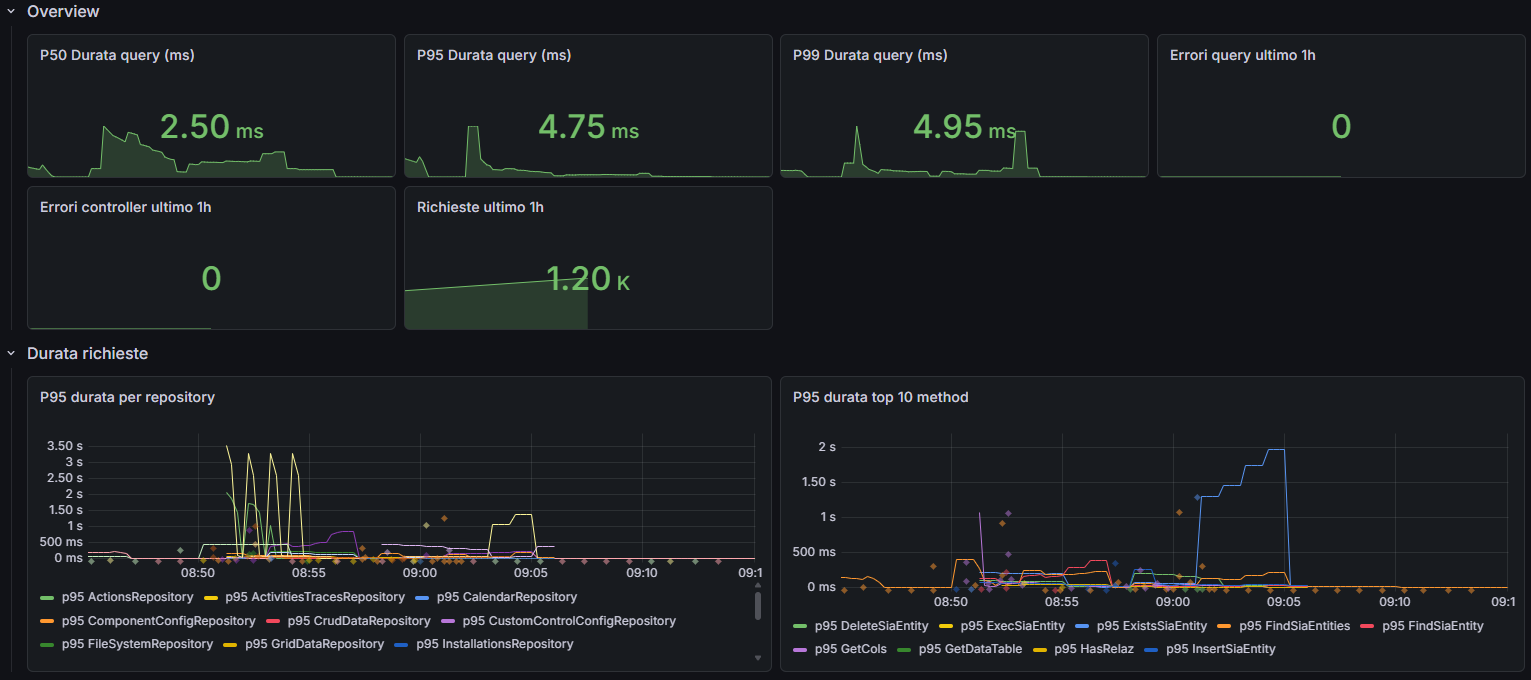
\includegraphics[width=1.25\textwidth]{../images/screenshots/DashboardBase.png}
    }
    \caption{Overview e durata richieste della dashboard di \emph{Sia.Base}}
    \label{fig:dash-base}
\end{figure}

\begin{figure}[h]
    \centering
    \makebox[\textwidth][c]{%
        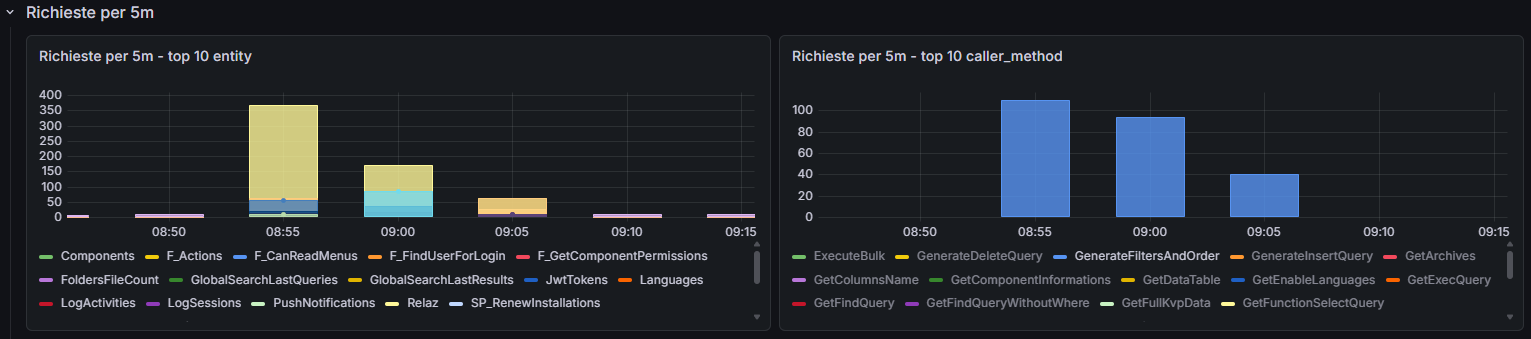
\includegraphics[width=1.25\textwidth]{../images/screenshots/DashboardBucket.png}
    }
        \caption{Sezione richieste per \texttt{\$\{bucket\}} della dashboard \emph{Sia.Base}}
    \label{fig:dash-bucket}
\end{figure}

\begin{figure}[h]
    \centering
    \makebox[\textwidth][c]{%
        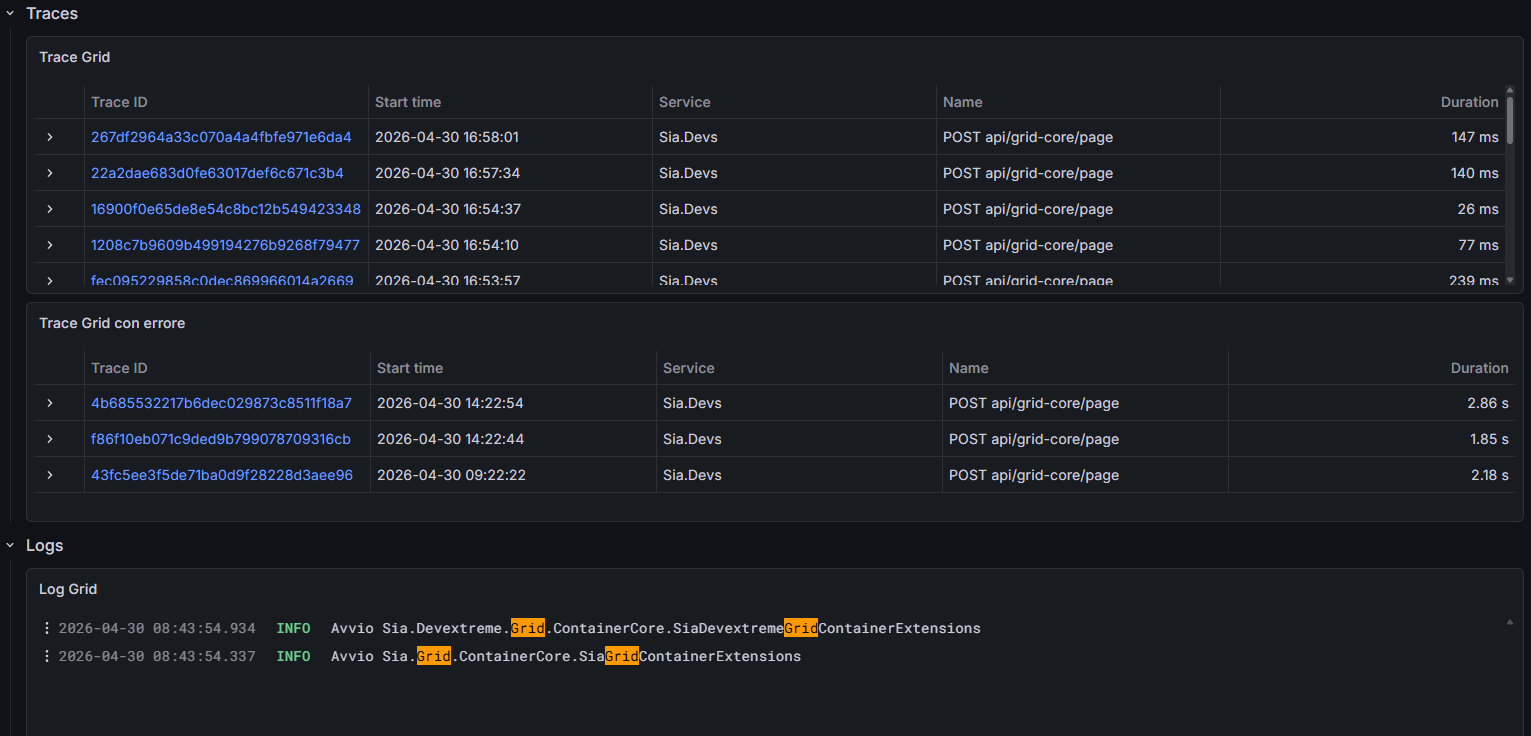
\includegraphics[width=1.25\textwidth]{../images/screenshots/DashboardLogsTrace.png}
    }
    \caption{Sezione trace e log della dashboard di \emph{Sia.Grid}}
    \label{fig:dash-logs-trace}
\end{figure}

\section{Telemetria delle performance hardware}

\subsection{Contesto e obiettivo}

Il modulo \texttt{Sia.HealthChecks.Servers} è parte del framework \emph{Sia.Server.Framework}
ed è responsabile della raccolta periodica di indicatori sullo stato del server che ospita
l'applicazione, con successiva notifica ad un \emph{manager} centrale delle installazioni.
Prima dell'intervento di telemetria, il modulo esponeva già i dati tramite:
\begin{itemize}
    \item cinque implementazioni di \texttt{IHealthCheck} (\texttt{CpuUsageHealthCheck},\\
        \texttt{CpuTemperatureHealthCheck}, \texttt{RamHealthCheck}, \texttt{DiskHealthCheck},
        \texttt{SqlHealthCheck}), invocate dall'endpoint \texttt{/health} di ASP.NET Core;
    \item un \texttt{BackgroundService} (\texttt{HealthCheckServerHostedService}) che, ad
        intervallo configurabile (\texttt{HealthNotifyDelayMinutes}), aggrega i risultati e
        invia il report al \emph{manager} tramite un \texttt{HttpClient} dedicato
        (\texttt{HealthCheckServerToServerApi}).
\end{itemize}

\subsection{Scelte progettuali}

Il modulo presenta due caratteristiche che lo distinguono dagli altri moduli instrumentati.

La prima è l'assenza di un controller: gli \texttt{IHealthCheck} sono invocati
dall'infrastruttura ASP.NET Core, non da endpoint applicativi. Di conseguenza
\texttt{SiaHealthChecksServersDiagnostics} non implementa \texttt{IControllerDiagnostics}
e non espone il counter \texttt{ControllerErrors}.

La seconda è la natura \emph{istantanea} dei dati raccolti. CPU\%, temperatura, GB di
RAM liberi e spazio su disco non sono grandezze cumulative: l'uso di \texttt{Counter} o
\texttt{Histogram} sarebbe improprio. Lo strumento corretto è l'\texttt{ObservableGauge},
la cui callback viene invocata on-demand al momento dello \emph{scrape} di Prometheus.
Poiché le letture hardware avvengono solo quando l'endpoint \texttt{/health} viene
interrogato, le gauge leggono un valore \textbf{in cache}, aggiornato dagli
\texttt{IHealthCheck} alla loro esecuzione, evitando di esporre dati stantii.

\subsection{Segnali prodotti}

\subsubsection{Trace}

Il modulo produce tre span custom, organizzate gerarchicamente.

\begin{table}[h]
\centering
\caption{Span prodotte dal modulo \texttt{Sia.HealthChecks.Servers}}
\label{tab:span-healthchecks}
\begin{tabularx}{\textwidth}{|l|X|X|}
\hline
\textbf{Span} & \textbf{Contesto} & \textbf{Tag principali} \\
\hline
\texttt{...cycle} & Root span di ogni iterazione del \texttt{HostedService}
  & \texttt{sia.enabled}, \texttt{sia.delay\_minutes}, \texttt{sia.success},
    \texttt{exception.type} \\
\hline
\texttt{...check} & Child span per ogni \texttt{IHealthCheck} invocato
  & \texttt{sia.check}, \texttt{sia.status}, \texttt{sia.caller\_method} \\
\hline
\texttt{...send} & Span attorno alla chiamata di invio al \emph{manager}
  & \texttt{sia.server\_id}, \texttt{sia.result}, \texttt{exception.type} \\
\hline
\end{tabularx}
\end{table}

Le trace HTTP generate automaticamente da \texttt{HttpClient} restano figlie di
\texttt{...send}, permettendo di ispezionare nella stessa trace sia la logica
applicativa sia il dettaglio del POST verso il manager.

\subsubsection{Metriche}

Accanto alle metriche cumulative standard (cycle, check, send), il modulo espone sei
\texttt{ObservableGauge} per i valori hardware istantanei.

\begin{table}[h]
\centering
\caption{ObservableGauge del modulo \texttt{Sia.HealthChecks.Servers}}
\label{tab:gauge-healthchecks}
\begin{tabular}{|l|c|p{7cm}|}
\hline
\textbf{Metrica} & \textbf{Unità} & \textbf{Descrizione} \\
\hline
\texttt{...cpu.usage}        & \%    & Percentuale di utilizzo della CPU al momento dell'ultima lettura \\
\hline
\texttt{...cpu.temperature}  & °C    & Temperatura del processore rilevata dai sensori hardware \\
\hline
\texttt{...ram.available}    & GByte & Memoria RAM libera disponibile per i processi \\
\hline
\texttt{...ram.total}        & GByte & Memoria RAM fisica totale installata nel server \\
\hline
\texttt{...disk.free}        & GByte & Spazio libero sul disco, distinto per \texttt{sia.drive} \\
\hline
\texttt{...disk.total}       & GByte & Capacità totale del disco, distinta per \texttt{sia.drive} \\
\hline
\end{tabular}
\end{table}

I tag hanno domini piccoli e chiusi (\texttt{sia.check} $\in \{cpu,\allowbreak\ cpu\_temperature,\allowbreak\ ram,\allowbreak\ disk,\allowbreak\ sql\}$,
\texttt{sia.status} $\in \{Healthy, Unhealthy\}$), mantenendo la cardinalità sotto
controllo indipendentemente dal numero di installazioni monitorate.

\subsection{Dashboard Grafana}

La dashboard segue lo schema standard del progetto, con l'aggiunta di una riga
\emph{Risorse} dedicata alle gauge hardware: andamento di CPU\% e temperatura nel tempo,
RAM disponibile confrontata a soglia, spazio disco libero per drive e una \emph{state
timeline} delle connessioni SQL che visualizza a colpo d'occhio gli intervalli in cui una
connessione è risultata \emph{down}. I pannelli trace e log consentono, a partire da un
picco anomalo su qualsiasi metrica hardware, di navigare alla trace del ciclo di notifica
corrispondente e ai log emessi in quell'iterazione, chiudendo il percorso diagnostico
metrica $\rightarrow$ trace $\rightarrow$ log.

\begin{figure}[h]
    \centering
    \makebox[\textwidth][c]{%
        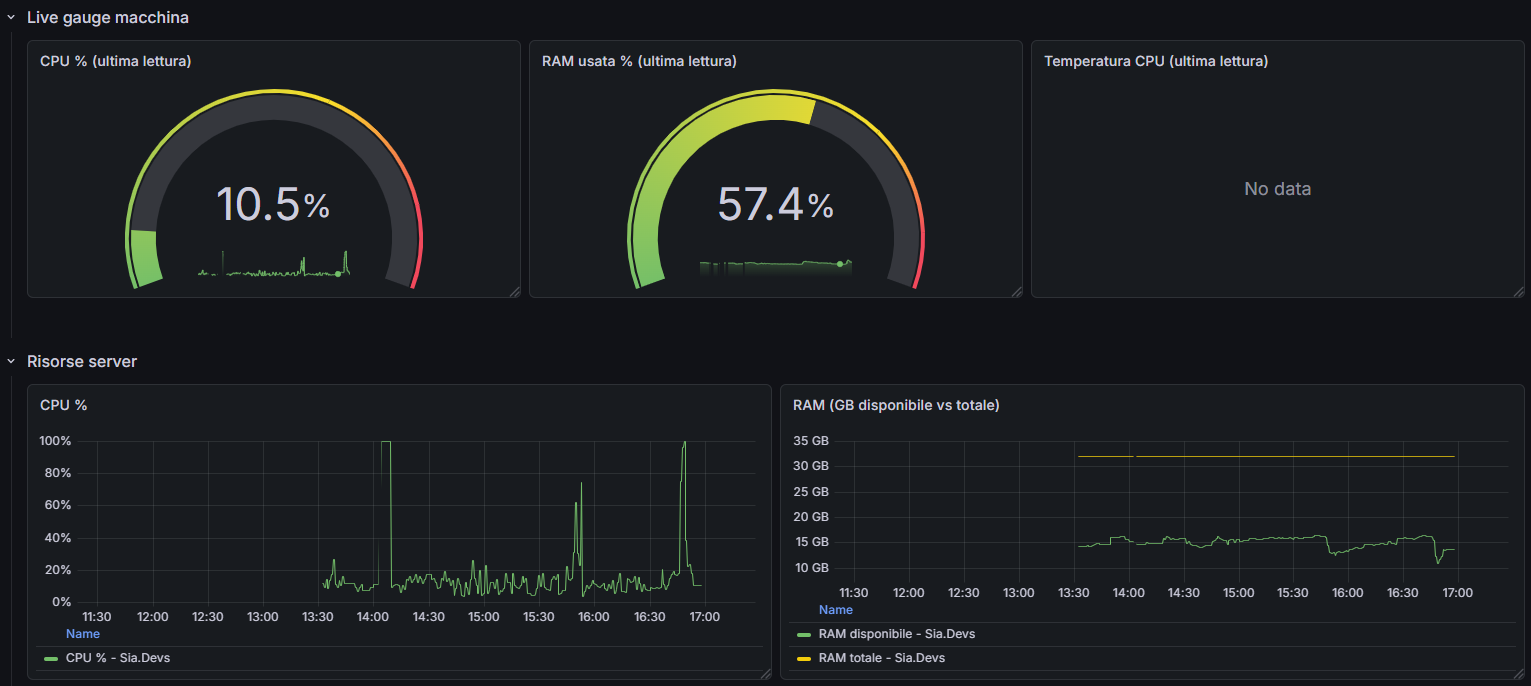
\includegraphics[width=1.25\textwidth]{../images/screenshots/DashboardHardware.png}
    }
    \caption{Sezione risorse della dashboard di telemetria hardware}
    \label{fig:dash-hardware-telemetry}
\end{figure}